% Provenance (never printed): see sources/outline_sources.md (Year 1: stress and
% principal stresses in 2D; strain; pure and simple shear; elastic, brittle and ductile
% behaviour; the strength envelope of the lithosphere). Strength envelopes from
% figdata/bachelor-1/strength_envelope.py (Byerlee 1975; flow laws of Gleason and Tullis
% 1995 and Hirth and Kohlstedt 2003 as compiled by Lopez-Sanchez; geotherms of ch. 10);
% exercise and problem values in the Book 3 scratch calculator calc/ch16.py. Traction,
% shear stress, the stress and strain tensors, Hooke's law, Young's modulus and viscosity
% belong to the physics series and are recalled, never defined (sync 1 ruling).
\chapter{应力、应变与流变学}\label{ch:b1:stress-strain-rheology}

20世纪60年代，美国丹佛附近的落基山兵工厂将废液注入一口处置井，
废液扩散到地表以下的破碎结晶基底中，深度介于
\qty{3.7}{km} 至 \qty{7.0}{km} 之间，随后发生了地震。
地震都局限在岩石中流体压力升高超过
约 \qty{3.2}{MPa} 的部分。
% ledger: hb81:denver
半个世纪后，类似的事情在俄克拉何马州以更大的规模重演：
那里与石油、天然气一同采出的含盐水被重新压回地下。在
该州及周边地区，震级为 3 级或以上的地震，
2005 至 2008 年间每年只有 1 至 5 次，2009 年为 \num{20} 次，2014 年为 \num{585} 次，
2015 年为 \num{888} 次，平均每天超过两次；震级为 5.7 和 5.8 的两次地震先后袭击了
布拉格（2011 年）和帕尼（2016 年）。仅四口大注水量的处置井
就可能导致美国中部地震总数的五分之一，并
使其中一些地震发生在 \qty{30}{km} 以外。
% ledger: usgs:oklahoma-rate, usgs:prague-pawnee, keranen:oklahoma
注水并没有把岩石推开，只是提高了
岩石孔隙中流体的压力。为什么这会使断层滑动？
答案需要三个概念，它们正是本章的主题：岩石内某一平面上的
应力，岩石在何种条件下沿该平面破坏，
以及孔隙流体的压力会抵消把两侧压在一起的力。
借助这三个概念，并结合热岩石的蠕变定律，
便能画出整个\omterm{def:b1:layered-earth:lithosphere}{岩石圈}强度随深度变化的曲线。

\begin{recall}
作用在面上的力，通过其单位面积上的力来描述，单位为帕斯卡；
静止流体中的压强随深度按 $\rho g z$ 增大（见物理学教材）。
弹簧以及小形变中的固体服从胡克定律：应变与应力成正比，
比例常数为杨氏模量；黏性流体的阻力与其剪切速率成正比，
比例常数为动力黏度。
物理学教材的大学三年级分册用张量描述三维的应力与应变，
本章只需要二维情形。对称的 $2\times2$ 矩阵有两个
实特征值和两个相互垂直的
特征向量（数学，一年级）。\omterm{def:b1:heat-budget:geotherm}{地温线}见
\cref{ch:b1:heat-budget}，它给出了深度处的温度；断层在
第 1 册七年级时已经学过。
\end{recall}

\section{二维应力}\label{sec:b1:stress-strain-rheology:stress}

设想沿一个小的平面将岩石切开。切面一侧的岩石以一定的力
压向另一侧的岩石，单位面积上的这个力称为该面上的面力，
这是物理学教材中的用语。它的方向一般
并不沿该面的法线方向。

\begin{definition}[法向应力]\label{def:b1:stress-strain-rheology:stress}
岩石中某点的某一平面上，一侧岩石对另一侧施加的单位面积力，
沿该平面法线方向有一个分量，
称为\emph{法向应力}\index{法向应力} $\sigma_n$，沿平面方向有一个分量，
即切应力 $\tau$。在地球科学中，法向应力
压缩时取正值。
\end{definition}

这一符号约定与工程师的相反。之所以这样选取，
是因为固体地球中几乎所有应力都是压应力：
上覆岩石的重量压在其下的一切之上。

我们在竖直平面内讨论，取水平方向为 $x$ 轴，竖直方向为 $y$ 轴。
在与 $x$ 轴垂直的面上，\omterm{def:b1:stress-strain-rheology:stress}{法向应力}为 $\sigma_{xx}$，切应力为
$\sigma_{xy}$；在与 $y$ 轴垂直的面上，二者分别为 $\sigma_{yy}$
与 $\sigma_{yx}$。两个切应力相等：对于一个小正方形，
竖直两边上的剪切力构成力偶，
力矩为 $\sigma_{xy}a\cdot a$（$a$ 为边长）；水平两边上的剪切力构成
反向的力偶，力矩为 $\sigma_{yx}a\cdot a$。若二者不等，正方形就会
发生转动。因此，一点处的应力只需三个数即可描述，
它们足以给出任一平面上的应力。

\begin{proposition}[斜面上的应力]\label{prop:b1:stress-strain-rheology:transformation}
设某平面的单位法向量为 $\vec n = (\cos\theta, \sin\theta)$，
夹角 $\theta$ 自 $x$ 轴量起，并设 $\vec m = (-\sin\theta, \cos\theta)$
为沿该平面的单位向量。该面上的\omterm{def:b1:stress-strain-rheology:stress}{法向应力}与切应力为
\begin{align*}
  \sigma_n &= \sigma_{xx}\cos^2\theta + 2\sigma_{xy}\sin\theta\cos\theta + \sigma_{yy}\sin^2\theta
           = \frac{\sigma_{xx}+\sigma_{yy}}{2} + \frac{\sigma_{xx}-\sigma_{yy}}{2}\cos2\theta + \sigma_{xy}\sin2\theta, \\
  \tau     &= (\sigma_{yy}-\sigma_{xx})\sin\theta\cos\theta + \sigma_{xy}(\cos^2\theta - \sin^2\theta)
           = -\frac{\sigma_{xx}-\sigma_{yy}}{2}\sin2\theta + \sigma_{xy}\cos2\theta ,
\end{align*}
其中 $\tau$ 沿 $\vec m$ 方向取正值。
\end{proposition}

\begin{proof}
取一个小棱柱，如下图所示：一个
面积为 $A$、外法线为 $\vec n$ 的斜面，一个竖直面，
面积为 $A\cos\theta$，一个水平面，面积为 $A\sin\theta$，均为单位长度（第三方向）上的面积。
棱柱的重量与惯性正比于其体积，
而体积的缩小快于其表面积；因此对于足够小的棱柱，各面上的力自身必须平衡。
取压应力为正，棱柱外的岩石
在竖直面上施加的力为
$A\cos\theta\,(\sigma_{xx}, \sigma_{xy})$，在水平面上施加的力为
$A\sin\theta\,(\sigma_{xy}, \sigma_{yy})$；在斜面上施加的力为
$-A(\sigma_n\vec n + \tau\vec m)$。三者之和为零：
\[
  \sigma_n\vec n + \tau\vec m = \cos\theta\,(\sigma_{xx}, \sigma_{xy}) + \sin\theta\,(\sigma_{xy}, \sigma_{yy}) .
\]
与 $\vec n$ 作数量积得到 $\sigma_n$，与 $\vec m$ 作数量积得到 $\tau$，
因为 $\vec n\cdot\vec m = 0$。第二种形式由
$\cos^2\theta = (1+\cos2\theta)/2$，$\sin^2\theta = (1-\cos2\theta)/2$ 以及
$2\sin\theta\cos\theta = \sin2\theta$ 得到。
\end{proof}

\begin{omfigure}
\begin{tikzpicture}[>={Stealth[length=5pt]}, font=\small]
% theta = 35 deg, hypotenuse L = 4.5: a = L cos(theta), b = L sin(theta)
\pgfmathsetmacro{\th}{35}
\pgfmathsetmacro{\L}{4.5}
\pgfmathsetmacro{\a}{\L*cos(\th)}
\pgfmathsetmacro{\b}{\L*sin(\th)}
\coordinate (O) at (0,0);
\coordinate (A) at (0,\a);
\coordinate (B) at (\b,0);
\coordinate (M) at ($(A)!0.5!(B)$);
\fill[omLithGranite!45] (O) -- (A) -- (B) -- cycle;
\draw[line width=0.8pt] (O) -- (A) -- (B) -- cycle;
% axes
\draw[->, black!70] (-2.6,-1.9) -- (-1.6,-1.9) node[right] {$x$};
\draw[->, black!70] (-2.6,-1.9) -- (-2.6,-0.9) node[above] {$y$};
% face on x = 0 (outward normal -x), area A cos(theta)
\draw[->, line width=1.1pt, omDef] (-1.35,0.5*\a) -- (-0.05,0.5*\a);
\node[omDef, anchor=south] at (-0.95,0.5*\a+0.05) {$\sigma_{xx} A\cos\theta$};
\draw[->, line width=1.1pt, omProp] (-0.25,0.5*\a-1.25) -- (-0.25,0.5*\a-0.25);
\node[omProp, anchor=east] at (-0.3,0.5*\a-0.85) {$\sigma_{xy} A\cos\theta$};
% face on y = 0 (outward normal -y), area A sin(theta)
\draw[->, line width=1.1pt, omDef] (0.68*\b,-1.35) -- (0.68*\b,-0.05);
\node[omDef, anchor=west] at (0.68*\b+0.05,-1.05) {$\sigma_{yy} A\sin\theta$};
\draw[->, line width=1.1pt, omProp] (0.1,-0.25) -- (1.1,-0.25);
\node[omProp, anchor=north east] at (0.9,-0.32) {$\sigma_{xy} A\sin\theta$};
% inclined face, area A, normal n = (cos theta, sin theta)
\draw[->, line width=1.1pt, omThm] ($(M)+(\th:1.5)$) -- ($(M)+(\th:0.05)$);
\node[omThm, anchor=south west, inner sep=1pt] at ($(M)+(\th:1.5)$) {$\sigma_n A$};
\draw[->, line width=1.1pt, omThm!70!black] ($(M)+(\th:0.25)+(\th-90:0.75)$) -- ($(M)+(\th:0.25)+(\th-90:1.75)$);
\node[omThm!70!black, anchor=west] at ($(M)+(\th:0.3)+(\th-90:1.3)$) {$\tau A$};
\draw[->, black!70, dashed] ($(M)+(\th+90:1.25)$) -- ++(\th:1.0) node[pos=1, anchor=south west, inner sep=1pt, text=black] {$\boldsymbol n$};
% angle theta at A, between the face and the y axis
\pic[draw, angle radius=0.75cm, pic text={$\theta$}, angle eccentricity=1.35] {angle = O--A--B};
\end{tikzpicture}
\par\smallskip{\small 作用于一个小三角棱柱岩石上的力的平衡。斜面面积为 $A$，
单位法向量为 $\vec n$；竖直面与水平面的面积分别为
$A\cos\theta$ 与 $A\sin\theta$。蓝色：两个小面上的法向力；
橙色：其上的剪切力；红色：斜面上的法向力与
剪切力。压应力取正，因此所有法向力都指向
棱柱内部。}
\label{fig:b1:stress-strain-rheology:prism}
\end{omfigure}

\begin{theorem}[主应力]\label{thm:b1:stress-strain-rheology:principal}
岩石中每一点处都存在两个互相垂直的平面，其上的剪应力
为零。这两个平面上的\omterm{def:b1:stress-strain-rheology:stress}{法向应力}，分别是过该点所有平面上
\omterm{def:b1:stress-strain-rheology:stress}{法向应力}的最大值与最小值，
\[
  \sigma_{1,3} = \frac{\sigma_{xx}+\sigma_{yy}}{2} \pm
  \sqrt{\Bigl(\frac{\sigma_{xx}-\sigma_{yy}}{2}\Bigr)^2 + \sigma_{xy}^2},
  \qquad \tan2\theta_p = \frac{2\sigma_{xy}}{\sigma_{xx}-\sigma_{yy}},
\]
其中 $\theta_p$ 为从 $x$ 轴到
承载 $\sigma_1$ 的平面法线的夹角。
\end{theorem}

\begin{proof}
记 $c = (\sigma_{xx}+\sigma_{yy})/2$，取 $R \ge 0$ 与 $\theta_p$，
使 $(\sigma_{xx}-\sigma_{yy})/2 = R\cos2\theta_p$ 且
$\sigma_{xy} = R\sin2\theta_p$，则
$R = \sqrt{((\sigma_{xx}-\sigma_{yy})/2)^2 + \sigma_{xy}^2}$，且
$\tan2\theta_p$ 如上所述。
\cref{prop:b1:stress-strain-rheology:transformation} 的第二种形式化为
\[
  \sigma_n = c + R\cos(2\theta - 2\theta_p), \qquad \tau = -R\sin(2\theta - 2\theta_p).
\]
\omterm{def:b1:stress-strain-rheology:stress}{法向应力}的最大值为 $c + R$，在 $\theta = \theta_p$ 处取得，最小值
$c - R$，在 $\theta = \theta_p + \ang{90}$ 处取得；两处均有 $\tau = 0$。另请注意
$\mathrm d\sigma_n/\mathrm d\theta = 2\tau$，即\omterm{def:b1:stress-strain-rheology:stress}{法向应力}
恰在剪应力为零处取驻值。
\end{proof}

\begin{definition}[主应力，差应力]\label{def:b1:stress-strain-rheology:principal}
称某点处的\emph{主应力}\index{主应力}为
两个无剪应力平面上的\omterm{def:b1:stress-strain-rheology:stress}{法向应力} $\sigma_1 \ge \sigma_3$，
其方向称为主方向。在三维情形中
共有三个，$\sigma_1 \ge \sigma_2 \ge \sigma_3$，分别位于三个
互相垂直的平面上。\emph{差应力}\index{差应力 }
 为 $\sigma_1 - \sigma_3$，平面内的平均应力为
$(\sigma_1+\sigma_3)/2$。
\end{definition}

应力状态在其主方向上最易读懂。若
将角 $\theta$ 从 $\sigma_1$ 的方向量起，而非从
$x$ 轴量起，则公式的最后几项消失。

\begin{proposition}[莫尔圆]\label{prop:b1:stress-strain-rheology:mohr}
对平面，以 $\theta$ 记其法线与
$\sigma_1$ 方向的夹角，则
\[
  \sigma_n = \frac{\sigma_1+\sigma_3}{2} + \frac{\sigma_1-\sigma_3}{2}\cos2\theta,
  \qquad
  |\tau| = \frac{\sigma_1-\sigma_3}{2}\,|\sin2\theta| .
\]
随 $\theta$ 变化，点 $(\sigma_n, |\tau|)$ 描出一个圆的上半部分，
该圆圆心为 $((\sigma_1+\sigma_3)/2,\, 0)$，半径为
$(\sigma_1-\sigma_3)/2$，角度为 $2\theta$，自其 $\sigma_1$ 端量起。
最大剪应力 $(\sigma_1-\sigma_3)/2$ 作用于与主方向成
\ang{45} 角的平面上。
\end{proposition}

\begin{proof}
在主轴方向上，$\sigma_{xx} = \sigma_1$，$\sigma_{yy} = \sigma_3$，且
$\sigma_{xy} = 0$，由\cref{prop:b1:stress-strain-rheology:transformation}
可得两式。于是
$(\sigma_n - (\sigma_1+\sigma_3)/2)^2 + \tau^2 = ((\sigma_1-\sigma_3)/2)^2$，此为圆的方程；
$|\sin2\theta|$ 在 $\theta = \ang{45}$ 时最大。
\end{proof}

$\tau$ 的符号仅说明两侧将沿哪一方向滑动，因此
通常只画圆的上半部分。该作图以
工程师克里斯蒂安·奥托·莫尔命名，他还在此基础上建立了一个
破坏判据，这也是下面要讨论的内容
（见\cref{sec:b1:stress-strain-rheology:rheology}）。

\subsection*{深度处的应力}

\begin{definition}[静岩压力，孔隙流体压力，有效应力]\label{def:b1:stress-strain-rheology:lithostatic}
在深度 $z$ 处，单位水平面积上方岩石的重量
即竖向应力 $\sigma_v = \int_0^z\rho g\,\mathrm dz'$，
在密度均匀的层中为 $\rho g z$，其中 $\rho$ 为密度。
当各方向应力相同且都等于它时，岩石承受\emph{静岩
压力}\index{静岩压力}。岩石孔隙与裂隙中水、油或气体的
压力即\emph{孔隙流体
压力}\index{孔隙流体压力} $P$；它为静力的，
即 $P = \rho_w g z$，当孔隙与地表连通时。
\emph{有效应力}\index{有效应力}为应力减去
孔隙压力，即在每个平面上 $\sigma' = \sigma - P$；$\lambda = P/\sigma_v$ 为
孔隙压力比。
\end{definition}

在密度为 \qty{2700}{kg.m^{-3}} 的\omterm{def:b1:layered-earth:layers}{地壳}中，竖向应力每千米增加
$2700\times9.81\times1000 = \qty{26.5}{MPa}$，而静力的孔隙压力
每千米增加 \qty{9.81}{MPa}，$\lambda = 1000/2700 = 0.37$。
孔隙流体以各方向相同的压力将颗粒推开，
它不改变剪应力，但会从每个\omterm{def:b1:stress-strain-rheology:stress}{法向应力}中减去 $P$。
例如孔隙被黏土或盐封闭时，
流体可承担上覆岩石的部分重量，$\lambda$ 随之
上升并趋向 1。

\omterm{def:b1:layered-earth:layers}{地壳}中的应力并非\omterm{def:b1:stress-strain-rheology:lithostatic}{静岩压力}。板块推挤与拉伸，\omterm{def:b1:layered-earth:layers}{地壳}
发生弯曲，山脉的重量压在其根部，水平应力与
竖向应力不同。近地表处不承受剪应力，其中一个
主方向为竖直方向，如\cref{ch:b1:faults-folds-fabrics}所示：
$\sigma_v$ 为 $\sigma_1$、$\sigma_2$ 或 $\sigma_3$，三种情形即
断层运动的三种方式。

\section{应变}\label{sec:b1:stress-strain-rheology:strain}

应力是原因，应变是岩石所记录的结果。化石被拉长、
卵石被压扁、岩层缩短成\omterm{def:b1:geological-maps:fold}{褶皱}，都度量了形状的改变。

\begin{definition}[伸长率，伸长比，剪应变]\label{def:b1:stress-strain-rheology:strain}
长为 $\ell_0$ 的物质线变形为长度 $\ell$ 后，具有
\emph{伸长率}\index{伸长率} $e = (\ell - \ell_0)/\ell_0$，以及
\emph{伸长比}\index{伸长比} $S = \ell/\ell_0 = 1 + e$；缩短是
负的伸长率，伸长比小于 1。原本互相垂直的两条物质线
现夹角为 $\ang{90} - \psi$，已被剪切了角
$\psi$，则\emph{剪应变}\index{剪应变}为
$\gamma = \tan\psi$。
\end{definition}

当每一小块岩石都以相同的方式变形时，应变是均匀的。
$\vec x'$ 为点 $\vec x$ 的新位置，则它是
线性函数 $\vec x' = F\vec x$，其中常数 $2\times2$ 矩阵 $F$（且
$\det F > 0$，岩石不会翻转内外）。直线仍为直线，
平行线仍平行；正方形变为平行四边形，
圆变为椭圆。

\begin{proposition}[应变椭圆]\label{prop:b1:stress-strain-rheology:ellipse}
在均匀应变 $\vec x' = F\vec x$ 下，半径为 1 的圆
变为椭圆，其半轴 $S_1 \ge S_2$ 为
$FF^{\mathsf T}$ 的本征值的平方根，沿其互相垂直的特征向量方向。
$S_1$ 与 $S_2$ 分别是所有物质线中最大和最小的\omterm{def:b1:stress-strain-rheology:strain}{伸长比}，
面积乘以 $\det F = S_1S_2$。
\end{proposition}

\begin{proof}
点 $\vec x = F\vec u$ 来自圆上的点 $\vec u$，
$|\vec u| = 1$，故 $|F^{-1}\vec x|^2 = 1$，即
$\vec x^{\mathsf T}(FF^{\mathsf T})^{-1}\vec x = 1$。矩阵
$B = FF^{\mathsf T}$ 为对称矩阵，其本征值 $\lambda_1 \ge
\lambda_2$ 均为正（$\vec v^{\mathsf T}B\vec v = |F^{\mathsf T}\vec v|^2 > 0$）；在其
互相垂直的特征向量方向上，方程化为
$x_1^2/\lambda_1 + x_2^2/\lambda_2 = 1$，这是半轴为
$\sqrt{\lambda_1}$ 与 $\sqrt{\lambda_2}$ 的椭圆。物质线沿单位矢量
$\vec u$ 方向，其\omterm{def:b1:stress-strain-rheology:strain}{伸长比}为 $|F\vec u|$，
且 $|F\vec u|^2 = \vec u^{\mathsf T}F^{\mathsf T}F\vec u$ 介于
$F^{\mathsf T}F$ 的本征值之间，而这些与 $FF^{\mathsf T}$ 的相同。最后，
$\lambda_1\lambda_2 = \det B = (\det F)^2$。
\end{proof}

\begin{definition}[应变椭圆]\label{def:b1:stress-strain-rheology:strain-ellipse}
\emph{应变椭圆}\index{应变椭圆}是均匀应变把
半径为 1 的圆变成的椭圆；其半轴为
主\omterm{def:b1:stress-strain-rheology:strain}{伸长比} $S_1 \ge S_2$，其轴为
应变的主方向。
\end{definition}

使物体形状发生同样改变的两种应变，可以截然不同。

\begin{definition}[纯剪切，简单剪切]\label{def:b1:stress-strain-rheology:shear-types}
\emph{纯剪切}\index{纯剪切}是保持面积的均匀应变，
且其主方向在岩石中保持固定：
在这些轴上 $F = \begin{pmatrix} k & 0 \\ 0 & 1/k\end{pmatrix}$，
其中 $k > 1$。\emph{简单剪切}\index{简单剪切}使每一点
沿某一方向（即剪切方向）平行移动，移动量为 $\gamma$ 乘以该点
到一个与之平行的固定平面的距离：
$F = \begin{pmatrix} 1 & \gamma \\ 0 & 1\end{pmatrix}$。
\end{definition}

两者都保持面积，因为两个行列式都为 1。在\omterm{def:b1:stress-strain-rheology:shear-types}{纯剪切}中，
沿\omterm{def:b1:stress-strain-rheology:strain-ellipse}{应变椭圆}轴的物质线在每个阶段都是同一条线，
即应变是共轴的。在\omterm{def:b1:stress-strain-rheology:shear-types}{简单剪切}中则不然，如
下一命题及其后的图所示。

\begin{proposition}[简单剪切的椭圆]\label{prop:b1:stress-strain-rheology:simple-shear}
\omterm{def:b1:stress-strain-rheology:shear-types}{简单剪切} $\gamma$ 的主\omterm{def:b1:stress-strain-rheology:strain}{伸长比}为
\[
  S_{1,2} = \sqrt{1 + \gamma^2/4} \pm \gamma/2 ,
\]
其\omterm{def:b1:stress-strain-rheology:strain-ellipse}{应变椭圆}的长轴与剪切方向所成的角
$\theta'$，由 $\tan2\theta' = 2/\gamma$ 给出。
\end{proposition}

\begin{proof}
$FF^{\mathsf T} = \begin{pmatrix} 1+\gamma^2 & \gamma \\ \gamma & 1\end{pmatrix}$
其迹为 $2+\gamma^2$，行列式为 1。故 $S_1S_2 = 1$，
且 $S_1^2 + S_2^2 = 2 + \gamma^2$，从而 $(S_1 - S_2)^2 = \gamma^2$，
$S_1 - S_2 = \gamma$，于是 $S_1 = \gamma/2 + \sqrt{1+\gamma^2/4}$。
一个对称矩阵的最大本征值所对应的特征向量，
$\begin{pmatrix} a & b \\ b & d\end{pmatrix}$ 与第一坐标轴所成的角由 $\tan2\theta' = 2b/(a-d)$ 给出
（与\cref{thm:b1:stress-strain-rheology:principal}是同一计算）：
此处为 $2\gamma/\gamma^2 = 2/\gamma$。
\end{proof}

\begin{omfigure}
\begin{tikzpicture}[>={Stealth[length=4.5pt]}, font=\small, scale=0.95]
% unit square [-1,1]^2 with its inscribed circle, mapped by exact linear maps (cm = a,b,c,d: x' = a x + c y, y' = b x + d y)
% pure shear: diag(k, 1/k), k = (1 + sqrt 5)/2 = 1.618; simple shear: gamma = 1, S1 = 1.618, long axis at 31.72 deg
\pgfmathsetmacro{\k}{(1+sqrt(5))/2}
\pgfmathsetmacro{\ik}{1/\k}
% (a) undeformed
\begin{scope}
  \fill[omLithSand!70] (-1,-1) rectangle (1,1);
  \draw[line width=0.7pt] (-1,-1) rectangle (1,1);
  \draw[line width=0.9pt, omDef] (0,0) circle[radius=1];
  \draw[omThm, line width=0.6pt] (-1,-1) -- (1,1);
  \draw[omProp, line width=0.6pt] (-1,1) -- (1,-1);
  \node[font=\small\bfseries] at (0,-1.55) {(a) 变形前};
\end{scope}
% (b) pure shear
\begin{scope}[xshift=4.2cm]
  \draw[black!35, dashed] (-1,-1) rectangle (1,1);
  \begin{scope}[cm={\k,0,0,\ik,(0,0)}]
    \fill[omLithSand!70] (-1,-1) rectangle (1,1);
    \draw[line width=0.7pt] (-1,-1) rectangle (1,1);
    \draw[line width=0.9pt, omDef] (0,0) circle[radius=1];
    \draw[omThm, line width=0.6pt] (-1,-1) -- (1,1);
    \draw[omProp, line width=0.6pt] (-1,1) -- (1,-1);
  \end{scope}
  \draw[omDef, dashed] (-\k,0) -- (\k,0);
  \draw[omDef, dashed] (0,-\ik) -- (0,\ik);
  \draw[->, line width=0.8pt] (1.72,0) -- (2.15,0);
  \draw[->, line width=0.8pt] (-1.72,0) -- (-2.15,0);
  \draw[->, line width=0.8pt] (0,1.2) -- (0,0.72);
  \draw[->, line width=0.8pt] (0,-1.2) -- (0,-0.72);
  \node[font=\small\bfseries] at (0,-1.55) {(b) 纯剪切};
\end{scope}
% (c) simple shear, gamma = 1
\begin{scope}[xshift=9.0cm]
  \draw[black!35, dashed] (-1,-1) rectangle (1,1);
  \begin{scope}[cm={1,0,1,1,(0,0)}]
    \fill[omLithSand!70] (-1,-1) rectangle (1,1);
    \draw[line width=0.7pt] (-1,-1) rectangle (1,1);
    \draw[line width=0.9pt, omDef] (0,0) circle[radius=1];
    \draw[omThm, line width=0.6pt] (-1,-1) -- (1,1);
    \draw[omProp, line width=0.6pt] (-1,1) -- (1,-1);
  \end{scope}
  % long and short axes of the strain ellipse: S1 = 1.618 at 31.72 deg, S2 = 0.618 at 121.72 deg
  \draw[omDef, dashed] (211.72:\k) -- (31.72:\k);
  \draw[omDef, dashed] (121.72:\ik) -- (301.72:\ik);
  \draw[->, line width=0.8pt] (-1.2,1.3) -- (0.8,1.3);
  \draw[->, line width=0.8pt] (1.2,-1.3) -- (-0.8,-1.3);
  \draw[black!60] (-2,-1) -- (-2,0.2);
  \draw[black!70] (-2,-0.3) arc[start angle=90, end angle=45, radius=0.7];
  \node[font=\scriptsize] at ($(-2,-1)+(67.5:0.98)$) {$\psi$};
  \node[font=\small\bfseries] at (0,-1.75) {(c) 简单剪切};
\end{scope}
\end{tikzpicture}
\par\smallskip{\small 带内切圆的岩石方块（a），分别经
\omterm{def:b1:stress-strain-rheology:shear-types}{纯剪切}（$k = 1.618$，b）和\omterm{def:b1:stress-strain-rheology:shear-types}{简单剪切}（$\gamma = 1$）变形
（c）后的情形，两者具有相同的主\omterm{def:b1:stress-strain-rheology:strain}{伸长比} 1.618 与 0.618。蓝色虚线：
\omterm{def:b1:stress-strain-rheology:strain-ellipse}{应变椭圆}的轴；灰色虚线：变形前的方块。在\omterm{def:b1:stress-strain-rheology:shear-types}{纯剪切}中，
轴始终位于同一条物质线上；在\omterm{def:b1:stress-strain-rheology:shear-types}{简单剪切}中，长轴
与剪切方向成 \ang{31.7}，而起初为伸长最快方向的对角线
（红色）已越过该轴，
转到 \ang{26.6}。图形是方块与圆在
两个矩阵作用下的精确像。}
\label{fig:b1:stress-strain-rheology:shear}
\end{omfigure}

\omterm{def:b1:stress-strain-rheology:strain-ellipse}{应变椭圆}记录的是总应变，即\emph{有限}应变。一段持续数百万年的变形
是许多小增量之和，每一增量都是一个无穷小应变；
当 $\gamma$ 较小时，命题给出
$S_{1,2} \approx 1 \pm \gamma/2$ 与 $\theta' \approx \ang{45}$。在\omterm{def:b1:stress-strain-rheology:shear-types}{简单
剪切}中，各增量总在与剪切方向成 \ang{45} 处伸长最快，
而有限\omterm{def:b1:stress-strain-rheology:strain-ellipse}{应变椭圆}向剪切方向转动，$\gamma = 1$ 时为 \ang{31.7}，
在 $\gamma = 2$ 时为 \ang{22.5}，且随 $\gamma$ 增大越来越接近剪切方向。这
是为什么强剪切带中压扁的卵石与拉长的\omterm{def:b1:rock-forming-minerals:mineral}{矿物}几乎位于带的平面之内，
也是为什么它们与该带所成的夹角可度量该带已移动了
多远。

\section{流变学}\label{sec:b1:stress-strain-rheology:rheology}

\begin{definition}[流变学、脆性行为与韧性行为]\label{def:b1:stress-strain-rheology:rheology}
材料的\emph{流变学}\index{流变学}，是指其在应力作用下变形与流动的方式，
即应力、应变及应变速率之间的关系。
岩石的变形表现为\emph{脆性行为}\index{脆性行为}时，
是通过断裂，或沿断裂面、在离散的面上滑动而变形，并伴随强度的突然丧失；
岩石表现出\emph{韧性行为}\index{韧性行为}时，
则是在其整个体积内持续而永久地变形，
且不丧失\omterm{def:b1:stress-strain-rheology:coulomb}{内聚力}。
\end{definition}

岩石表现出物理学教材中的全部行为。在微小而短暂的应力作用下，
它们呈弹性：应变与应力成正比，正如
胡克定律所述，并随应力的消失而消失；地震波
（见\cref{ch:b1:layered-earth}）即在弹性岩石中传播。长时间尺度上，
炽热的\omterm{def:b1:layered-earth:layers}{地幔}如同黏度极大的流体一样流动，应变速率随应力增大而增大；
二者之间，冷岩石会破裂并滑动，温岩石则缓慢蠕变。
哪种行为占主导，取决于应力、温度、压强、孔隙中的流体
以及作用持续的时间。

\subsection*{脆性破坏}

\begin{definition}[库仑破裂准则]\label{def:b1:stress-strain-rheology:coulomb}
岩石服从\emph{库仑破裂准则}\index{库仑破裂准则}，即
当穿过其中的某一平面发生破裂，或既有裂隙发生滑动时，
只要该平面上满足
\[
  \tau = C + \mu\,\sigma_n' , \qquad \sigma_n' = \sigma_n - P ,
\]
成立，其中 $C \ge 0$ 为岩石的\emph{内聚力}\index{内聚力}，
$\mu$ 为其\emph{内摩擦系数}\index{内摩擦系数}，而
$\phi = \arctan\mu$ 为其
\emph{内摩擦角}\index{内摩擦角}。
\end{definition}

该准则以库仑和莫尔之名命名。其中的常数由实验室中的样品测得，
因岩石而异。既有裂隙已丧失\omterm{def:b1:stress-strain-rheology:coulomb}{内聚力}，即 $C = 0$，其上的摩擦
几乎与岩石无关，
（见\cref{prop:b1:stress-strain-rheology:byerlee}）：$\mu$ 介于 0.6 与 0.85 之间，
摩擦角介于 \ang{31} 与
\ang{40} 之间。
% ledger: byerlee:1975

\begin{theorem}[破裂角]\label{thm:b1:stress-strain-rheology:failure-angle}
服从库仑准则的岩石首先在夹角为
$\ang{45} - \phi/2$（相对 $\sigma_1$ 方向）的平面上破裂，
两侧皆可，破裂条件为
\[
  \frac{\sigma_1' - \sigma_3'}{2} = C\cos\phi + \frac{\sigma_1' + \sigma_3'}{2}\,\sin\phi .
\]
\end{theorem}

\begin{proof}
作\omterm{def:b1:stress-strain-rheology:lithostatic}{有效应力}下的莫尔圆，圆心为 $c' =
(\sigma_1'+\sigma_3')/2$，半径为 $r = (\sigma_1'-\sigma_3')/2$
（见下图）。孔隙压强使该圆
整体平移了 $P$，因其从每个正应力中减去 $P$，而对剪应力无影响。
整个圆位于直线 $\tau = C + \mu\sigma_n'$ 之下时，
没有平面破裂。随应力变化，最先破裂的平面
对应圆与直线相切的点。该处半径与直线垂直，
直线的\omterm{def:b1:geological-maps:attitude}{倾角}为 $\phi$（相对水平方向），
故接触点处的半径夹角为 $\ang{90} + \phi$，此角自 $\sigma_1$ 端方向量起。
由\cref{prop:b1:stress-strain-rheology:mohr}可知，该点即法线与
$\theta$ 角（自 $\sigma_1$ 量起）的平面，其中 $2\theta = \ang{90} + \phi$；
该平面本身与 $\ang{90} - \theta = \ang{45} - \phi/2$ 角（相对 $\sigma_1$），
而圆的下半部分给出对称的平面。
接触意味着由圆心到直线的距离
等于半径：
$r = (C + \mu c')/\sqrt{1+\mu^2} = C\cos\phi + c'\sin\phi$，由于
$\cos\phi = 1/\sqrt{1+\mu^2}$ 与 $\sin\phi = \mu/\sqrt{1+\mu^2}$。
\end{proof}

\begin{omfigure}
\begin{tikzpicture}[>={Stealth[length=5pt]}, font=\small, x=0.072cm, y=0.072cm]
% C = 10 MPa, mu = 0.6 (phi = 30.96 deg), sigma_3' = 20 MPa; tangency r = (C + mu sigma_3') / (sqrt(1+mu^2) - mu)
\pgfmathsetmacro{\C}{10}
\pgfmathsetmacro{\mmu}{0.6}
\pgfmathsetmacro{\pphi}{atan(\mmu)}
\pgfmathsetmacro{\sth}{20}
\pgfmathsetmacro{\r}{(\C+\mmu*\sth)/(sqrt(1+\mmu*\mmu)-\mmu)}
\pgfmathsetmacro{\c}{\sth+\r}
\pgfmathsetmacro{\sone}{\c+\r}
\pgfmathsetmacro{\tf}{90+\pphi}
% axes
\draw[->] (-8,0) -- (122,0) node[below left] {$\sigma_n'$};
\draw[->] (0,-6) -- (0,80) node[left] {$\tau$};
% the upper half of the circle (tau >= 0)
\draw[line width=0.9pt, omDef] (\c+\r,0) arc[start angle=0, end angle=180, radius=\r];
\fill (\c,0) circle[radius=0.9pt];
\node[below, font=\scriptsize] at (\c,-1) {$\frac{\sigma_1'+\sigma_3'}{2}$};
\fill (\sth,0) circle[radius=1.1pt] node[below left, inner sep=1.5pt] {$\sigma_3'$};
\fill (\sone,0) circle[radius=1.1pt] node[below right, inner sep=1.5pt] {$\sigma_1'$};
% Coulomb envelope
\draw[line width=0.9pt, omThm] (0,\C) -- (116,\C+116*\mmu) node[above left, align=right, font=\scriptsize] {库仑包络线 \\ $\tau = C + \mu\,\sigma_n'$};
\fill[omThm] (0,\C) circle[radius=1.1pt] node[left] {$C$};
\draw[dashed, black!60] (0,\C) -- (30,\C);
\draw[black!70] (18,\C) arc[start angle=0, end angle=\pphi, radius=18];
\node[font=\scriptsize] at (22,\C+5.3) {$\phi$};
% the failure point T, at 2 theta = 90 + phi from the sigma_1 end
\coordinate (T) at ({\c+\r*cos(\tf)},{\r*sin(\tf)});
\draw[black!70] (\c,0) -- (T);
\fill[omThm] (T) circle[radius=1.5pt];
\node[anchor=south east, font=\scriptsize, align=right, inner sep=1pt] at ($(T)+(-1,1)$) {破裂的平面：\\ $2\theta = 90^\circ + \phi$};
% right angle between radius and envelope
\coordinate (Ta) at ($(T)!2.5mm!(\c,0)$);
\coordinate (Tb) at ($(T)!2.5mm!(116,\C+116*\mmu)$);
\draw[black!70] (Ta) -- ($(Ta)+(Tb)-(T)$) -- (Tb);
% a general plane: 2 theta = 50 deg
\coordinate (P) at ({\c+\r*cos(50)},{\r*sin(50)});
\draw[omProp, dashed] (\c,0) -- (P);
\fill[omProp] (P) circle[radius=1.5pt] node[above right, inner sep=1.5pt] {$(\sigma_n', \tau)$};
\draw[omProp, dotted] (P) -- (P |- 0,0);
\draw[omProp] (\c+9,0) arc[start angle=0, end angle=50, radius=9];
\node[omProp, font=\scriptsize] at ({\c+13.5*cos(25)},{13.5*sin(25)}) {$2\theta$};
\end{tikzpicture}
\par\smallskip{\small \omterm{def:b1:stress-strain-rheology:lithostatic}{有效应力}下的莫尔圆与库仑包络线。
法线与 $\theta$ 角（自 $\sigma_1$ 量起）的平面，对应于
$2\theta$ 角（自 $\sigma_1$ 端起算）的点（橙色）。所画的圆恰好与
包络线相切：切点处的平面发生破裂，其法线的夹角
$\theta = \ang{45} + \phi/2$（自 $\sigma_1$ 量起），该处半径与包络线垂直。按比例绘制，取
$C = \qty{10}{MPa}$，
$\mu = 0.6$ 与 $\sigma_3' = \qty{20}{MPa}$，由此得
$\sigma_1' = \qty{97.7}{MPa}$。}
\label{fig:b1:stress-strain-rheology:mohr}
\end{omfigure}

当 $\phi = \ang{30}$ 时，岩石沿与 $\sigma_1$ 成 \ang{30} 的平面破裂，
两个可能的破裂面彼此成 \ang{60} 夹角，
且 $\sigma_1$ 将此夹角平分。这正是野外所见共轭断层之间的夹角，
也解释了如\cref{ch:b1:faults-folds-fabrics}所示的
正断层\omterm{def:b1:geological-maps:attitude}{倾角}陡而逆冲断层\omterm{def:b1:geological-maps:attitude}{倾角}缓的原因。

对于已有裂隙上的滑动，实验直接给出了摩擦本身，
且其规律出人意料地简单。

\begin{proposition}[拜尔利定律]\label{prop:b1:stress-strain-rheology:byerlee}
对于大多数岩石，已存在的裂隙或断层开始滑动的条件是剪应力
达到下列关系：
\[
  \tau = 0.85\,\sigma_n' \quad (\sigma_n' < \qty{200}{MPa}), \qquad
  \tau = \qty{50}{MPa} + 0.6\,\sigma_n' \quad (\sigma_n' > \qty{200}{MPa}),
\]
无论何种岩石，此即\emph{拜尔利定律}\index{拜尔利定律}。
\end{proposition}
\admitted

该定律来自实验，而非理论。詹姆斯·拜尔利于
1975 年测定了一块砂岩在围压与孔隙压力下的破裂强度与摩擦强度，
并发现二者均仅由\omterm{def:b1:stress-strain-rheology:lithostatic}{有效应力}决定，
即两种压力之差；破裂强度
随颗粒间胶结物而变化，幅度可达 \qty{20}{\percent}，而
摩擦强度与岩石种类无关，同一规律对辉长岩、
纯橄岩、蛇纹岩、花岗岩和石灰岩同样成立。两条直线相交于
$\sigma_n' = \qty{200}{MPa}$ 处，二者均给出 \qty{170}{MPa}。
% ledger: byerlee:1975

\omterm{def:b1:stress-strain-rheology:lithostatic}{有效应力}定律是本章开篇的关键。提高
孔隙压力升高 $\Delta P$，会使每个有效\omterm{def:b1:stress-strain-rheology:stress}{法向应力}降低
$\Delta P$，而剪应力保持不变：莫尔圆向左平移，
大小不变，朝破裂线靠近。原本稳定的断层
可在构造应力不变的情况下被诱发滑动。
断层的临界剪应力为 $\tau_c = \tau_0 + \mu(\sigma_n - P)$，
注入作用于其最后一项。在丹佛，地震只发生在
孔隙压力升高超过约 \qty{3.2}{MPa} 的岩石中，
仿佛该升高正是那里断层所需要的。
% ledger: hb81:denver

\begin{method}[检验断层是否滑动]\label{met:b1:stress-strain-rheology:slip-test}
判断深度 $z$ 处的断层是否会滑动，以及何种条件使其滑动：
\begin{enumerate}
  \item 求断层\omterm{def:b1:geological-maps:attitude}{走向}垂直面内的\omterm{def:b1:stress-strain-rheology:principal}{主应力}：
        竖向应力 $\sigma_v = \rho g z$，以及水平应力（可实测或假定）；
        取孔隙压力 $P$，
        若无其他信息，则取静水压力 $\rho_w g z$。
  \item 测量 $\theta$ 角，即断层法线与
        $\sigma_1$ 方向之间的夹角。
  \item 利用
        \cref{prop:b1:stress-strain-rheology:mohr}计算断层面上的 $\sigma_n$ 与 $\tau$，
        再求 $\sigma_n' = \sigma_n - P$。
  \item 将 $\tau$ 与
        \cref{prop:b1:stress-strain-rheology:byerlee}给出的摩擦强度比较：若低于该值，断层保持稳定；
        以 $\tau/\sigma_n'$ 与 0.85 比较，即可衡量安全裕度。
  \item 使断层开始滑动所需的孔隙压力升高量为
        $\Delta P = \sigma_n' - \tau/0.85$，适用于定律的低应力段，
        高应力段则为 $\sigma_n' - (\tau - 50)/0.6$（单位为兆帕）。
\end{enumerate}
\end{method}

\subsection*{韧性蠕变}

高温岩石不会等到破裂。在富含石英的岩石中，温度超过数百度，
而在\omterm{def:b1:rock-forming-minerals:groups}{橄榄石}中则需更高温度，晶体借缺陷的缓慢运动而变形，
缺陷穿过其晶格，岩石以
随应力与温度急剧增大的速率蠕变。

\begin{proposition}[幂律蠕变]\label{prop:b1:stress-strain-rheology:creep}
在高温下，以位错蠕变变形的岩石以应变
速率流动：
\[
  \dot\varepsilon = A\,(\sigma_1 - \sigma_3)^n \exp\Bigl(-\frac{E + PV}{RT}\Bigr),
\]
其中 $T$ 为热力学温度，$P$ 为压强，$R$ 为
气体常数，$A$、$n$、$E$（活化能）与 $V$（活化体积）为材料常数，
由实验室测定。要以
速率 $\dot\varepsilon$ 流动，需要的\omterm{def:b1:stress-strain-rheology:principal}{差应力}为
\[
  \sigma_1 - \sigma_3 = \Bigl(\frac{\dot\varepsilon}{A}\Bigr)^{1/n}
  \exp\Bigl(\frac{E + PV}{nRT}\Bigr).
\]
\end{proposition}
\admitted

该定律背后的机制属于本科三年级分册的内容。其
常数来自实验：对于湿石英岩，$n = 4$，
$E = \qty{223}{kJ.mol^{-1}}$ 及 $A = \num{1.1e-4}$（应力单位为兆帕，
时间单位为秒），取自 Gleason 与 Tullis（1995）；对于干\omterm{def:b1:rock-forming-minerals:groups}{橄榄石}，
$n = 3.5$，$E = \qty{530}{kJ.mol^{-1}}$，$V = \qty{18}{cm^3.mol^{-1}}$ 及
$A = \num{e5}$，取自 Hirth 与 Kohlstedt（2003）；$R =
\qty{8.314462618}{J.mol^{-1}.K^{-1}}$。
% ledger: lopez:flow-laws, codata:R
该定律有两个特征塑造了\omterm{def:b1:layered-earth:lithosphere}{岩石圈}。应力对速率的依赖很弱：
速率快十倍，石英岩只需增加 $10^{1/4} = 1.78$ 倍应力。
而应力对温度的依赖极强：指数项使
石英岩的强度每升高一百度即降低数倍。
自然界的应变速率很慢。一条宽 \qty{300}{km} 的\omterm{def:b1:layered-earth:layers}{地壳}带，
每年吸收 \qty{1}{cm} 的板块运动，其变形速率为
$0.01/(\num{3.16e7}\times\num{3e5}) \approx \qty{1e-15}{s^{-1}}$，
即本书所用的速率。

\begin{inthelab}[测量岩石强度]
\begin{minipage}[t]{0.58\linewidth}\vspace{0pt}
岩石力学实验室在三轴压力室中测定强度。圆柱形
岩样经取芯并将两端磨平，装入橡胶或软金属制成的护套中，
护套可阻止围压流体进入孔隙。岩样置于一个厚壁压力容器中：
周围的油设定围压，
围压即 $\sigma_2 = \sigma_3$；活塞作用于岩样两端，
施加轴向荷载 $\sigma_1$。另有一条管路以独立压力向孔隙充水，
使\omterm{def:b1:stress-strain-rheology:lithostatic}{有效应力}可在总应力保持不变时改变。
试验机记录轴向力与样品的缩短量，
加载以恒定速率进行，直至样品破裂；
对于预先切开的样品，则直至切口开始滑动。炉子
置于容器内，用于加热蠕变实验的样品，这类实验
的应变速率比地球中的任何速率快出许多个数量级，因此必须
外推至地球条件。
\end{minipage}\hfill
\begin{minipage}[t]{0.38\linewidth}\vspace{0pt}
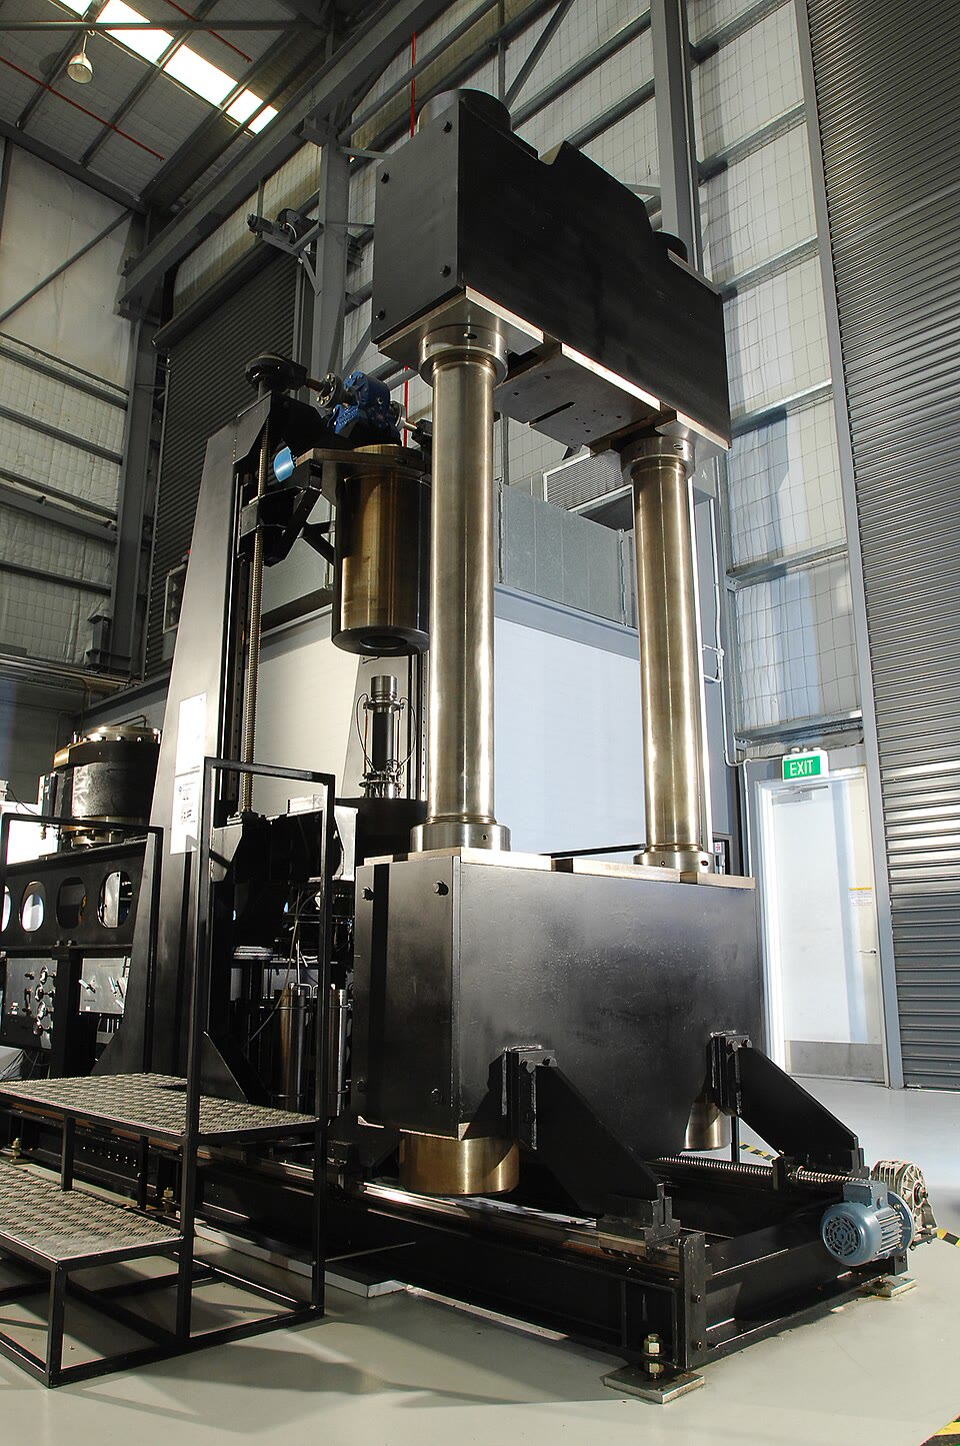
\includegraphics[width=\linewidth]{images/book3/b1-triaxial-cell.jpg}

{\scriptsize 用于测量岩石强度的高压三轴试验仪
（Darryl Peroni，CSIRO，CC BY 3.0）。}
% ledger: commons:csiro-triaxial
\end{minipage}
\end{inthelab}

\section{岩石圈的强度}\label{sec:b1:stress-strain-rheology:envelope}

在每一深度上，\omterm{def:b1:layered-earth:lithosphere}{岩石圈}可能以两种方式破坏：沿断层滑动，
其强度随有效压力增大；或发生蠕变，
其强度随温度升高而降低。\omterm{def:b1:layered-earth:lithosphere}{岩石圈}以
所需应力较小的方式变形。

\begin{definition}[强度包络线、脆–韧性转换带、孕震层]\label{def:b1:stress-strain-rheology:strength-envelope}
\omterm{def:b1:layered-earth:lithosphere}{岩石圈}的\emph{强度包络线}\index{强度包络线}是
给定应变速率下，岩石所能承受的最大\omterm{def:b1:stress-strain-rheology:principal}{差应力}随深度变化的曲线：
在每一深度上，取摩擦强度与蠕变强度中的较小者。
\emph{脆–韧性转换带}\index{脆–韧性转换带}
是两者相等的深度：在其上，岩石以断层方式变形，
在其下，以蠕变方式变形。\emph{孕震
层}\index{孕震层}
是大多数地震开始发生的深度范围。
\end{definition}

\begin{proposition}[摩擦强度随深度的变化]\label{prop:b1:stress-strain-rheology:brittle-gradient}
设某层密度为 $\rho$，孔隙压力为静水压力，
其中一个\omterm{def:b1:stress-strain-rheology:principal}{主应力}为竖直方向，断层取各种方向且无\omterm{def:b1:stress-strain-rheology:coulomb}{内聚力}，
摩擦系数为 $\mu$，则滑动开始时的\omterm{def:b1:stress-strain-rheology:principal}{差应力}为
\begin{align*}
  \sigma_1 - \sigma_3 &= \frac{2\mu}{\sqrt{1+\mu^2} + \mu}\,\rho g z(1-\lambda)
  && \text{若 $\sigma_v = \sigma_1$}, \\
  \sigma_1 - \sigma_3 &= \frac{2\mu}{\sqrt{1+\mu^2} - \mu}\,\rho g z(1-\lambda)
  && \text{若 $\sigma_v = \sigma_3$},
\end{align*}
其中 $\lambda = \rho_w/\rho$；第一种情形对应正断层，
第二种情形对应逆冲断层。
\end{proposition}

\begin{proof}
竖直\omterm{def:b1:stress-strain-rheology:lithostatic}{有效应力}为 $S = \rho g z - \rho_w g z = \rho g z(1-\lambda)$。
取 $C = 0$，$k = \sqrt{1+\mu^2}$，由\cref{thm:b1:stress-strain-rheology:failure-angle}
可知，当 $r = \mu c'/k$ 时断层发生滑动，其中 $r$ 为半径，$c'$ 为
有效莫尔圆的圆心。若 $\sigma_v = \sigma_1$，则
$\sigma_1' = S$ 且 $c' = S - r$，于是 $rk = \mu S - \mu r$，
$r = \mu S/(k+\mu)$。若 $\sigma_v = \sigma_3$，则 $c' = S + r$，
$r = \mu S/(k-\mu)$。\omterm{def:b1:stress-strain-rheology:principal}{差应力}为 $2r$。
\end{proof}

取 $\mu = 0.85$，$\rho = \qty{2700}{kg.m^{-3}}$，则 $S$ 每千米增加
\qty{16.7}{MPa}；摩擦强度在伸展条件下每千米增加
\qty{13.1}{MPa}，挤压条件下则每千米增加 \qty{61.3}{MPa}，
约为前者的近五倍，由此可见\omterm{def:b1:layered-earth:layers}{地壳}被拉开远比被推拢容易。
当有效\omterm{def:b1:stress-strain-rheology:stress}{法向应力}超过
\qty{200}{MPa} 时，\omterm{prop:b1:stress-strain-rheology:byerlee}{拜尔利定律}的上段起作用，挤压条件下的斜率
降至每千米约 \qty{35}{MPa}。
% computed in figdata/bachelor-1/strength_envelope.py (tested); ledger: byerlee:1975

\begin{omfigure}
\begin{tikzpicture}
\pgfplotsset{envaxis/.style={omrecord, omdepth, scale only axis, width=5.6cm, height=7.2cm,
  xmin=-1000, xmax=2500, ymin=0, ymax=80, xtick={-1000,0,1000,2000},
  ytick={0,10,...,80}, unbounded coords=jump,
  xlabel={差应力 $\sigma_1-\sigma_3$ (MPa)},
  tick label style={font=\scriptsize}, label style={font=\small},
  scaled x ticks=false, xticklabel style={/pgf/number format/.cd, 1000 sep={\,}}}}
% computed in figdata/bachelor-1/strength_envelope.py; ledger: byerlee:1975, lopez:flow-laws, codata:R, prem:moho-average
\begin{axis}[envaxis, name=cont, ylabel={深度 (km)}, title={\small (a) 大陆，\qty{55}{mW.m^{-2}}}]
\addplot[fill=omLithGranite!45, draw=none] table[x=x, y=depth] {figdata/out/bachelor-1-strength_envelope-continental-outline.dat};
\addplot[omThm, line width=0.5pt, restrict x to domain=-1:2450] table[x=thrust, y=depth] {figdata/out/bachelor-1-strength_envelope-continental.dat};
\addplot[omThm, line width=0.5pt, restrict x to domain=-2450:1] table[x expr=-\thisrow{normal}, y=depth] {figdata/out/bachelor-1-strength_envelope-continental.dat};
\addplot[omDef, line width=0.5pt, restrict x to domain=-1:2450] table[x=ductile, y=depth] {figdata/out/bachelor-1-strength_envelope-continental.dat};
\addplot[omDef, line width=0.5pt, restrict x to domain=-2450:1] table[x expr=-\thisrow{ductile}, y=depth] {figdata/out/bachelor-1-strength_envelope-continental.dat};
\addplot[black, line width=1.0pt] table[x=x, y=depth] {figdata/out/bachelor-1-strength_envelope-continental-outline.dat};
\draw[black!60, dashed] (axis cs:-1000,35) -- (axis cs:2500,35);
\node[font=\scriptsize, anchor=south east] at (axis cs:2480,35) {莫霍面};
\draw[black, densely dotted] (axis cs:0,0) -- (axis cs:0,80);
\draw[black!70] (axis cs:660,13.7) -- (axis cs:1700,18) node[anchor=north, font=\scriptsize, align=center, text=black] {转换带 \\ \qty{14}{km}};
\draw[black!70] (axis cs:1870,44.6) -- (axis cs:1950,53) node[anchor=north, font=\scriptsize, align=center, text=black] {地幔 \\ 转换带};
\node[font=\scriptsize, anchor=north, omThm] at (axis cs:1500,3) {挤压};
\node[font=\scriptsize, anchor=north, omThm] at (axis cs:-560,3) {伸展};
\node[font=\scriptsize, anchor=west, omDef] at (axis cs:40,31) {湿石英};
\node[font=\scriptsize, anchor=west, omDef] at (axis cs:300,66) {干橄榄石};
\end{axis}
\begin{axis}[envaxis, at={(cont.east)}, anchor=west, xshift=0.6cm, yticklabels={}, title={\small (b) 洋底，年龄 \qty{60}{Ma}}]
\addplot[fill=omLithBasalt!45, draw=none] table[x=x, y=depth] {figdata/out/bachelor-1-strength_envelope-oceanic-outline.dat};
\addplot[omThm, line width=0.5pt, restrict x to domain=-1:2450] table[x=thrust, y=depth] {figdata/out/bachelor-1-strength_envelope-oceanic.dat};
\addplot[omThm, line width=0.5pt, restrict x to domain=-2450:1] table[x expr=-\thisrow{normal}, y=depth] {figdata/out/bachelor-1-strength_envelope-oceanic.dat};
\addplot[omDef, line width=0.5pt, restrict x to domain=-1:2450] table[x=ductile, y=depth] {figdata/out/bachelor-1-strength_envelope-oceanic.dat};
\addplot[omDef, line width=0.5pt, restrict x to domain=-2450:1] table[x expr=-\thisrow{ductile}, y=depth] {figdata/out/bachelor-1-strength_envelope-oceanic.dat};
\addplot[black, line width=1.0pt] table[x=x, y=depth] {figdata/out/bachelor-1-strength_envelope-oceanic-outline.dat};
\draw[black, densely dotted] (axis cs:0,0) -- (axis cs:0,80);
\draw[black!70] (axis cs:2003,38.2) -- (axis cs:1900,50) node[anchor=north, font=\scriptsize, align=center, text=black] {转换带 \\ \qty{38}{km}};
\node[font=\scriptsize, anchor=west, omDef] at (axis cs:300,66) {干橄榄石};
\end{axis}
\end{tikzpicture}
\par\smallskip{\small 应变速率为
\qty{e-15}{s^{-1}}时的\omterm{def:b1:stress-strain-rheology:strength-envelope}{强度包络线}。红色：\omterm{prop:b1:stress-strain-rheology:byerlee}{拜尔利定律}给出的摩擦强度，
孔隙压力取静水压力，分别为挤压（逆冲断层，右侧）和
伸展（正断层，左侧，以负值绘制）；蓝色为
大陆\omterm{def:b1:layered-earth:layers}{地壳}中湿石英岩与\omterm{def:b1:layered-earth:layers}{地幔}中干\omterm{def:b1:rock-forming-minerals:groups}{橄榄石}的蠕变强度；黑色轮廓及阴影为
各深度上二者中较小的强度，即岩石的强度。
(a) 大陆，地表\omterm{def:b1:heat-budget:heat-flow}{热流}为 \qty{55}{mW.m^{-2}}，
\omterm{def:b1:layered-earth:layers}{地壳}厚 \qty{35}{km}：上\omterm{def:b1:layered-earth:layers}{地壳}强，下\omterm{def:b1:layered-earth:layers}{地壳}弱，最上部\omterm{def:b1:layered-earth:layers}{地幔}强。
(b) 洋底，年龄为 \qty{60}{Ma}：单一的强层，
挤压条件下厚 \qty{38}{km}。}
\label{fig:b1:stress-strain-rheology:envelope}
\end{omfigure}

上图将两种\omterm{def:b1:layered-earth:lithosphere}{岩石圈}的强度放在一起比较。
对两种\omterm{def:b1:layered-earth:lithosphere}{岩石圈}分别作图。大陆的\omterm{def:b1:heat-budget:geotherm}{地温线}采用
\cref{ch:b1:heat-budget}中的\omterm{def:b1:heat-budget:geotherm}{地温线}，地表\omterm{def:b1:heat-budget:heat-flow}{热流}为 \qty{55}{mW.m^{-2}}，
\omterm{def:b1:layered-earth:layers}{地壳}为厚 \qty{35}{km} 的湿石英岩，其下为干\omterm{def:b1:rock-forming-minerals:groups}{橄榄石}；洋底
年龄为 \qty{60}{Ma}，采用同一章中的半空间\omterm{def:b1:heat-budget:geotherm}{地温线}，
自海底向下为\omterm{def:b1:rock-forming-minerals:groups}{橄榄石}。应变速率为
\qty{e-15}{s^{-1}}。\qty{35}{km} 为
大陆下\omterm{def:b1:layered-earth:discontinuity}{莫霍面}的平均深度，取自\cref{ch:b1:layered-earth}中的\omterm{def:b1:layered-earth:reference-model}{参考地球模型}。
% ledger: prem:moho-average

大陆之下，\omterm{def:b1:stress-strain-rheology:strength-envelope}{脆–韧性转换带}在压缩条件下位于 \qty{13.7}{km} 深处，
此处温度为 \qty{249}{\degreeCelsius}；在伸展条件下则位于 \qty{17.1}{km} 处。
\omterm{def:b1:layered-earth:layers}{地壳}更热则转换带上升，更冷则下沉，
因为在给定应力下蠕变律仅取决于温度。该转换带是\omterm{def:b1:layered-earth:layers}{地壳}中
最强的层位。
其下强度急剧下降：在\omterm{def:b1:layered-earth:discontinuity}{莫霍面}处，温度为 \qty{527}{\degreeCelsius}，
石英岩在 \qty{7.6}{MPa} 下即可流动，而同一温度下的\omterm{def:b1:rock-forming-minerals:groups}{橄榄石}
则需约 \qty{30000}{MPa} 的应力，远超摩擦强度，以至于
\omterm{def:b1:layered-earth:layers}{地幔}顶部又重新呈脆性。第二个转换带位于
压缩条件下 \qty{44.6}{km} 处。该模型的下\omterm{def:b1:layered-earth:layers}{地壳}是夹在两层强层之间的软层，
即“果冻三明治”。洋底之下，整个
\omterm{def:b1:layered-earth:lithosphere}{岩石圈}均为\omterm{def:b1:rock-forming-minerals:groups}{橄榄石}，强度随深度增加，直至单一转换带，位于
\qty{38.2}{km} 处，温度为 \qty{641}{\degreeCelsius}。
% computed in figdata/bachelor-1/strength_envelope.py (tested)

地震与大洋\omterm{def:b1:stress-strain-rheology:strength-envelope}{强度包络线}相符：在大洋板块内部，
地震所达深度处的温度为
\qtyrange{600}{800}{\degreeCelsius}，接近模型中单一转换带的 \qty{641}{\degreeCelsius}。
更深的地震仅发生在一个板块俯冲到另一个板块之下
的地方，深度可超过 \qty{700}{km}
（见\cref{ch:b1:active-margins}）。
% ledger: jackson:jelly, usgs:deepest

大陆\omterm{def:b1:layered-earth:layers}{地幔}是存在争议的部分。二十年左右
间，“果冻三明治”模型一直是主流观点，其依据是
干\omterm{def:b1:rock-forming-minerals:groups}{橄榄石}的实验室测量，以及若干被认为位于
\omterm{def:b1:layered-earth:discontinuity}{莫霍面}之下的地震。2002 年，James Jackson 主张应当放弃该模型：更精确的
深度资料表明，大陆地震局限于单一层位，
通常为上\omterm{def:b1:layered-earth:layers}{地壳}，有时为整个\omterm{def:b1:layered-earth:layers}{地壳}，其下\omterm{def:b1:layered-earth:layers}{地幔}中没有可信的
地震，即便在\omterm{def:b1:layered-earth:discontinuity}{莫霍面}温度仅为
\qtyrange{300}{500}{\degreeCelsius} 时亦然。少量水，即\omterm{def:b1:rock-forming-minerals:groups}{橄榄石}中百万分之几的水含量，
便足以使其强度大幅下降，而大陆\omterm{def:b1:layered-earth:layers}{地幔}可能正含有这一水量；
此时大陆的强度主要位于
\omterm{def:b1:layered-earth:layers}{地壳}之中。两种观点由相同规律得出不同的包络线，
区别在于\omterm{def:b1:layered-earth:discontinuity}{莫霍面}以下\omterm{def:b1:rock-forming-minerals:groups}{橄榄石}是干还是湿。
% ledger: jackson:jelly
无论哪种观点正确，包络线都是界限而非测量结果：
实验室规律被外推到应变速率相差多个数量级的范围，
其给出的峰值应力超过 1 吉帕，远高于
地震实际释放的 \qtyrange{1}{10}{MPa}。
% ledger: jackson:jelly

\section{练习}

\begin{exercise}[$\star$]\label{exo:b1:stress-strain-rheology:1}
取密度为 \qty{2700}{kg.m^{-3}} 的\omterm{def:b1:layered-earth:layers}{地壳}，并取 $g = \qty{9.81}{m.s^{-2}}$。
在深度 \qty{10}{km} 处，计算：(a) 竖直应力，(b) 静水
孔隙压力，(c) 竖直\omterm{def:b1:stress-strain-rheology:lithostatic}{有效应力}及
孔隙压力比 $\lambda$。
\end{exercise}

\begin{exercise}[$\star$]\label{exo:b1:stress-strain-rheology:2}
(a) 一岩层长 \qty{10}{km}，被拉伸至 \qty{13}{km}：求其伸长量
及其\omterm{def:b1:stress-strain-rheology:strain}{伸长比}。(b) 另一岩层长 \qty{10}{km}，被缩短至 \qty{7}{km}。
(c) 岩石中原本互相垂直的两条线，现在夹角为
\ang{60}：求其角剪切及\omterm{def:b1:stress-strain-rheology:strain}{剪应变}。
\end{exercise}

\begin{exercise}[$\star$]\label{exo:b1:stress-strain-rheology:3}
某点处 $\sigma_1 = \qty{100}{MPa}$，$\sigma_3 = \qty{40}{MPa}$。
(a) 画出莫尔圆。(b) 求最大切应力，它作用于哪些面上，
以及这些面上的\omterm{def:b1:stress-strain-rheology:stress}{法向应力}是多少？(c) 计算 $\sigma_n$
及 $\tau$，其中面法线与 $\sigma_1$ 的夹角为 \ang{30}。
\end{exercise}

\begin{exercise}[$\star$]\label{exo:b1:stress-strain-rheology:4}
某岩石的\omterm{def:b1:stress-strain-rheology:coulomb}{内聚力}为 \qty{10}{MPa}，\omterm{def:b1:stress-strain-rheology:coulomb}{内摩擦角}为
\ang{30}。(a) 岩石在与 $\sigma_1$ 成多大角度时破裂？两个可能的破裂面彼此
之间的夹角为多少？(b) 当
$\sigma_3' = \qty{20}{MPa}$ 时，多大的有效 $\sigma_1'$ 会使其破裂？
\end{exercise}

\begin{exercise}[$\star\star$]\label{exo:b1:stress-strain-rheology:5}
在坐标轴 $x$（水平）与 $y$（竖直）中，$\sigma_{xx} = \qty{60}{MPa}$，
$\sigma_{yy} = \qty{20}{MPa}$，$\sigma_{xy} = \qty{15}{MPa}$。(a) 计算
\omterm{def:b1:stress-strain-rheology:principal}{主应力}及角度 $\theta_p$。(b) 借助
\cref{prop:b1:stress-strain-rheology:transformation}验证，法线为
$\theta_p$ 的面上无切应力，\omterm{def:b1:stress-strain-rheology:stress}{法向应力}为 $\sigma_1$。(c) 该点处
最大切应力是多少？
\end{exercise}

\begin{exercise}[$\star\star$]\label{exo:b1:stress-strain-rheology:6}
某剪切带中岩石经\omterm{def:b1:stress-strain-rheology:shear-types}{简单剪切}变形，\omterm{def:b1:stress-strain-rheology:strain}{剪应变} $\gamma = 2$。(a) 计算
主\omterm{def:b1:stress-strain-rheology:strain}{伸长比}，以及\omterm{def:b1:stress-strain-rheology:strain-ellipse}{应变椭圆}长轴与剪切方向的
夹角。(b) 验证面积未发生变化。(c) 一条
原与剪切方向成 \ang{45} 的物质线，沿剪切指向上升，
求其现在的位置、\omterm{def:b1:stress-strain-rheology:strain}{伸长比}，并与(a)的结果比较。
\end{exercise}

\begin{exercise}[$\star\star$]\label{exo:b1:stress-strain-rheology:7}
在厚 \qty{200}{m} 的剪切带中，板岩中的\omterm{def:b1:spherical-astronomy:spherical-triangle}{小圆}斑已变为
轴比为 4:1 的椭圆。假设为\omterm{def:b1:stress-strain-rheology:shear-types}{简单剪切}，且面积不变。
(a) 求 $S_1$、$S_2$ 及 $\gamma$。(b) 长轴应与剪切带壁面成多大角度？
(c) 一侧壁面相对另一侧已移动
多远？
\end{exercise}

\begin{exercise}[$\star\star$]\label{exo:b1:stress-strain-rheology:8}
深度为 \qty{3}{km} 处的一条断层，位于密度为 \qty{2700}{kg.m^{-3}} 的\omterm{def:b1:layered-earth:layers}{地壳}中，
其承受\omterm{def:b1:stress-strain-rheology:stress}{法向应力} \qty{70}{MPa} 与切应力 \qty{30}{MPa}。
(a) 若孔隙压力为静水压力，它是否按\omterm{prop:b1:stress-strain-rheology:byerlee}{拜尔利定律}
滑动？(b) 若孔隙封闭且 $\lambda = 0.6$，情况如何？(c) 求
开始滑动时的 $\lambda$ 值。
\end{exercise}

\begin{exercise}[$\star\star$]\label{exo:b1:stress-strain-rheology:9}
利用湿石英岩的蠕变律（见\cref{prop:b1:stress-strain-rheology:creep}）。
(a) 应力需增大为原来的多少倍，才能使其流动快十倍？
(b) 在相同应变速率且 $V = 0$ 时，其强度
由 \qty{400}{\degreeCelsius} 降至 \qty{500}{\degreeCelsius} 时减小为原来的多少倍？(c) 试用
这两个结果说明，\omterm{def:b1:stress-strain-rheology:strength-envelope}{脆–韧性转换带}的深度
为何更多地取决于\omterm{def:b1:heat-budget:geotherm}{地温线}，而非应变速率。
\end{exercise}

\begin{exercise}[$\star\star\star$]\label{exo:b1:stress-strain-rheology:10}
 当竖向应力为 $\sigma_2$ 时，断层为走滑断层。假设
 则此时竖向\omterm{def:b1:stress-strain-rheology:lithostatic}{有效应力}为平均值 $(\sigma_1' + \sigma_3')/2$。
 (a) 证明：摩擦系数为 $\mu$、无\omterm{def:b1:stress-strain-rheology:coulomb}{内聚力}时，滑动开始于
 $\sigma_1 - \sigma_3 = 2\mu\,\rho g z(1-\lambda)/\sqrt{1+\mu^2}$。(b) 计算
 以兆帕每千米为单位的斜率，对 $\mu = 0.85$ 和
 $\rho = \qty{2700}{kg.m^{-3}}$，并说明它位于正断层与
 逆冲断层的斜率之间。(c) 将这三个斜率分别表示为
 竖向\omterm{def:b1:stress-strain-rheology:lithostatic}{有效应力}的倍数。
\end{exercise}

\begin{exercise}[$\star\star\star$]\label{exo:b1:stress-strain-rheology:11}
 将年龄为 \qty{60}{Ma} 的大洋\omterm{def:b1:layered-earth:lithosphere}{岩石圈}模拟为由
 \qty{1350}{\degreeCelsius} 冷却而成的半无限空间，表面温度为 \qty{0}{\degreeCelsius}，取
$\kappa = \qty{e-6}{m^2.s^{-1}}$: $T = \num{1350}\operatorname{erf}\bigl(z/(2\sqrt{\kappa t})\bigr)$.
 (a) 计算 $2\sqrt{\kappa t}$。(b) 求
 \qty{600}{\degreeCelsius} 和 \qty{800}{\degreeCelsius} 等温线的深度。(c) 大洋板块内部的地震
 可达的深度，即温度为
 \qtyrange{600}{800}{\degreeCelsius} 的深度。将其与本章大洋\omterm{def:b1:stress-strain-rheology:strength-envelope}{强度包络线}中的\omterm{def:b1:stress-strain-rheology:strength-envelope}{脆–韧性
 转换带}作比较，后者位于
 \qty{38.2}{km} 深、\qty{641}{\degreeCelsius} 处。
% ledger: jackson:jelly
\end{exercise}

\begin{exercise}[$\star\star\star$]\label{exo:b1:stress-strain-rheology:12}
 岩石中发育各种方向的裂隙，所有裂隙都包含
 $\sigma_2$ 的方向，无\omterm{def:b1:stress-strain-rheology:coulomb}{内聚力}，摩擦系数为 0.85。有效
 \omterm{def:b1:stress-strain-rheology:principal}{主应力}为 $\sigma_1' = \qty{110}{MPa}$ 和
 $\sigma_3' = \qty{20}{MPa}$。(a) 证明有些裂隙会发生滑动。(b) 求
 滑动裂隙与 $\sigma_1$ 夹角的范围，并指出
 位于范围中间的是哪一个角度。(c) $\sigma_1'$ 降至何值，
 在 $\sigma_3'$ 固定时，仍至少有一条裂隙发生滑动？
\end{exercise}

\section{问题：断层会滑动吗？}

\begin{problem}[{周末问题——深度五千米处正断层上的应力，
 其安全裕度，以及使其滑动的孔隙压强升高
 量}]
\label{pb:b1:stress-strain-rheology:1}
% values: calc/ch16.py; ledger: byerlee:1975, hb81:denver
 一条断层\omterm{def:b1:geological-maps:attitude}{走向}为南北向，向东倾斜 \ang{60}。一口注水井
 在深度 \qty{5.00}{km} 处与断层相交，所在\omterm{def:b1:layered-earth:layers}{地壳}的密度为
 \qty{2700}{kg.m^{-3}}，其孔隙与地表相连。井中的一次测量
 给出垂直于断层的水平应力，
 为 \qty{75.0}{MPa}；沿\omterm{def:b1:geological-maps:attitude}{走向}的水平应力介于它与竖向应力之间，
 因此该问题可在竖直的东西向平面内作二维处理。
 取 $g = \qty{9.81}{m.s^{-2}}$，水的密度为
 \qty{1000}{kg.m^{-3}}，并采用\omterm{prop:b1:stress-strain-rheology:byerlee}{拜尔利定律}。应力精确到
 \qty{0.01}{MPa}。

\medskip
\noindent\textbf{第一部分——应力状态。}
\begin{enumerate}
  \item 计算断层所在深度处的竖向应力。
  \item 计算该处的静力孔隙压强，并求比值 $\lambda$。
  \item 两个应力中哪一个是 $\sigma_1$，哪一个是 $\sigma_3$？此应力状态
        驱动的是哪一类断层？
  \item 计算\omterm{def:b1:stress-strain-rheology:principal}{差应力}，以及莫尔圆的
        圆心与半径。
  \item 计算有效\omterm{def:b1:stress-strain-rheology:principal}{主应力}，以及\omterm{def:b1:stress-strain-rheology:lithostatic}{有效应力}圆的
        圆心。
  \item 取 $x$ 轴水平向东、$y$ 轴竖直，写出三个
        分量 $\sigma_{xx}$、$\sigma_{yy}$、$\sigma_{xy}$。为何
        $\sigma_{xy}$ 为零？
\end{enumerate}

\medskip
\noindent\textbf{第二部分——断层面上的应力。}
\begin{enumerate}[resume]
  \item 在第 6 题的坐标系中给出断层的单位法向量，以及
        $\theta$ 为它与 $\sigma_1$ 的夹角。
  \item 计算断层面上的 $\sigma_n$ 和 $\tau$，
        利用\cref{prop:b1:stress-strain-rheology:transformation}。
  \item 用莫尔圆检验这两个数值：断层位于从 $\sigma_1$
        端起算的哪个角度上？
  \item 计算断层面上的有效\omterm{def:b1:stress-strain-rheology:stress}{法向应力}。
  \item 计算比值 $\tau/\sigma_n'$，并与 0.85 作比较。
  \item 在当前的有效\omterm{def:b1:stress-strain-rheology:stress}{法向应力}下，使断层滑动需要多大的
        切应力？它还差多少兆帕？
\end{enumerate}

\medskip
\noindent\textbf{第三部分——莫尔圆与\omterm{prop:b1:stress-strain-rheology:byerlee}{拜尔利定律}。}
\begin{enumerate}[resume]
  \item 按比例画出有效莫尔圆和拜尔利直线。
  \item 计算圆心到该直线的距离，并
        与半径作比较。岩石中是否有任何平面会滑动？
  \item 哪个平面最先滑动？给出它与 $\sigma_1$ 的夹角及其\omterm{def:b1:geological-maps:attitude}{倾角}。
  \item 利用\cref{prop:b1:stress-strain-rheology:brittle-gradient}，计算
        该深度下正断层开始滑动时的\omterm{def:b1:stress-strain-rheology:principal}{差应力}，并
        与 \qty{13.1}{MPa} 每千米的斜率作核对。
  \item 水平应力须降至多低，方位最有利的平面才会
        滑动？
  \item 水平应力须降至多低，本题中的断层才会滑动？解释
        为何这一数值更低。
\end{enumerate}

\medskip
\noindent\textbf{第四部分——注入。}
\begin{enumerate}[resume]
  \item 解释为什么孔隙压强升高 $\Delta P$ 会使\omterm{def:b1:stress-strain-rheology:lithostatic}{有效
        应力}圆向左平移 $\Delta P$，而半径保持不变。
  \item 计算使方位最有利的平面开始滑动所需的
        孔隙压强升高量。
  \item 井中充满了水。泵须在井口额外施加多大的
        压强，才能使断层处的孔隙压强升高该数值？
        这相当于多高的水柱？
  \item 若断层上的摩擦系数为 0.6 而非 0.85，则它是否
        已经在滑动？断层保持平静说明其
        摩擦系数是多少？
  \item 在何种比值 $\lambda$ 下，方位最有利的平面会滑动？
  \item 以兆帕为单位、保留一位小数，求使该断层
        滑动所需的孔隙压强升高量。
\end{enumerate}
\end{problem}
